\chapter{Marco teórico}
\label{ch:marco}

% -----------------------------------------------------------------------
\section{Plataforma hardware}
\label{sec:plataforma}

\subsection{Arquitectura RISC-V}

RISC-V es un ISA abierto, modular y libre de
regalías desarrollado en la Universidad de California, Berkeley~\cite{riscvspec}.
La especificación base RV32I define 40 instrucciones de 32 bits distribuidas en
seis formatos según la disposición de sus campos. El campo \texttt{opcode}
identifica el formato; \texttt{funct3} y \texttt{funct7} discriminan variantes
dentro del mismo opcode. La Figura~\ref{fig:formatos} muestra los seis formatos
base y cómo están estructurados. Además, dado que la arquitectura es modular,
sobre la base RV32I se añaden extensiones opcionales
que amplían el conjunto de instrucciones sin modificar la codificación base.

\begin{figure}[H]
    \centering
    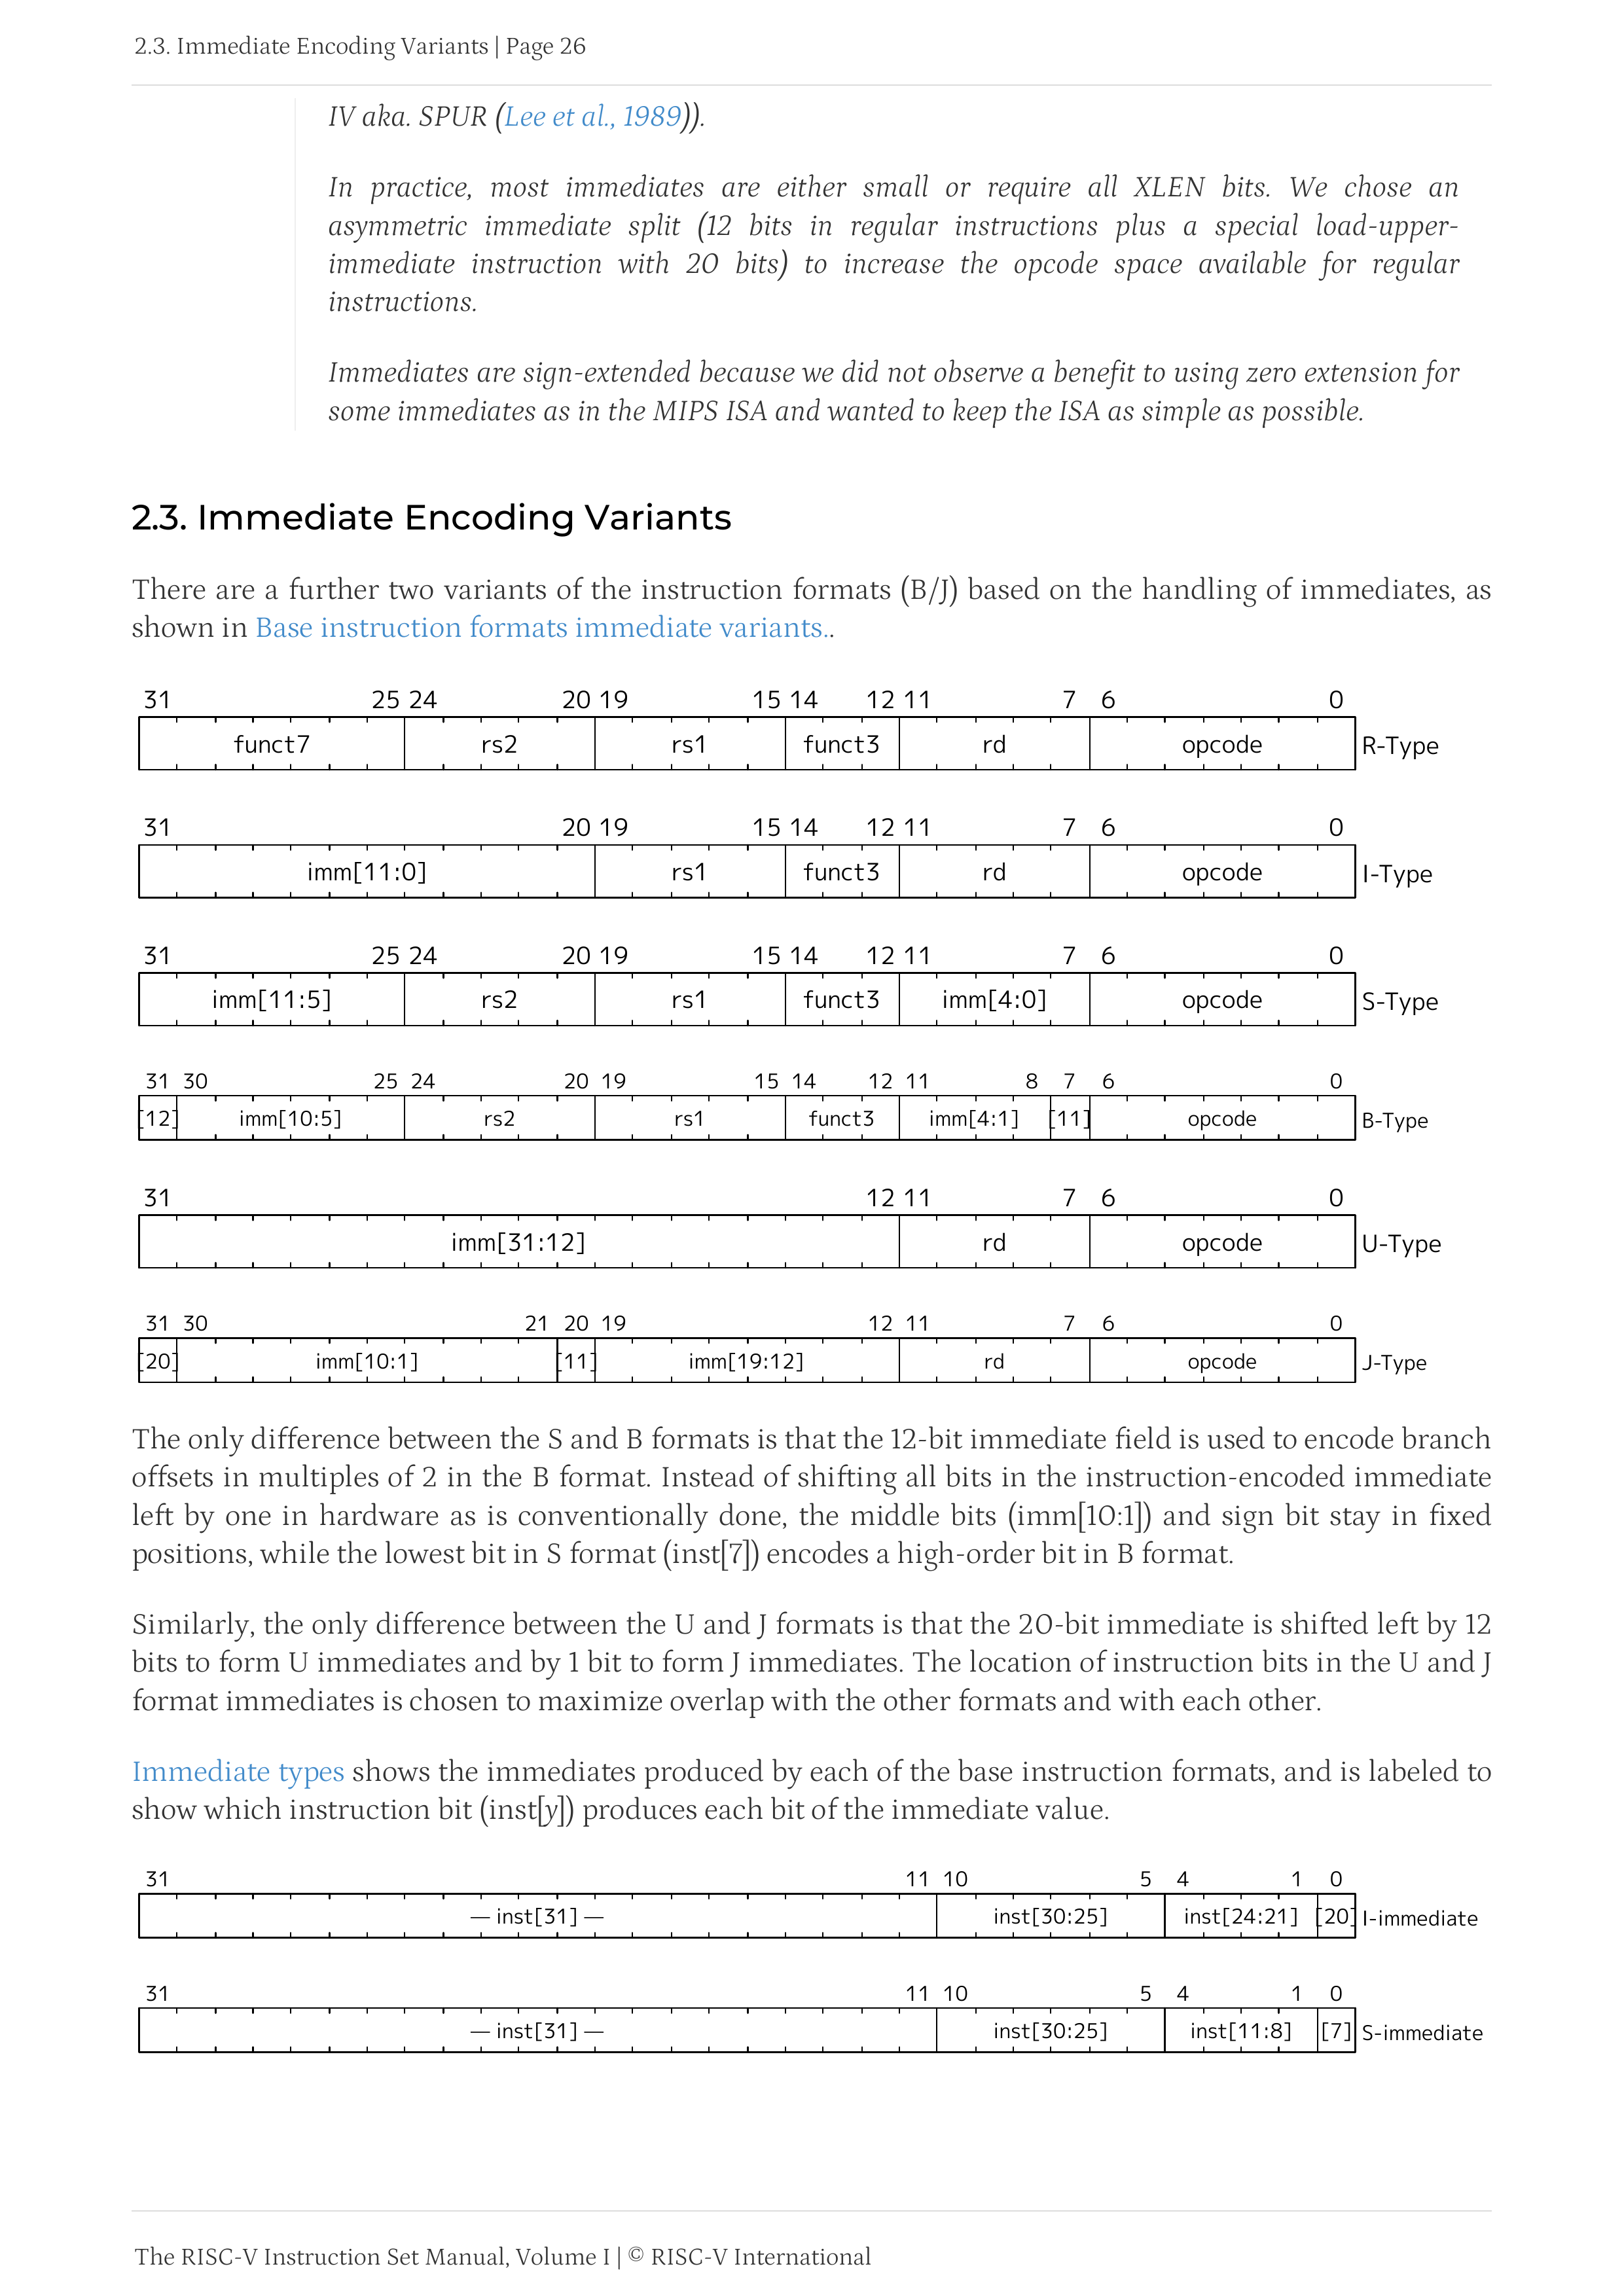
\includegraphics[trim=0.8cm 11.5cm 1.8cm 8.8cm, clip, width=\textwidth, height=0.30\textheight, keepaspectratio]{fig/riscv_formats_page-045.png}
    \caption{Formatos base de instrucción RISC-V RV32I~\cite{riscvspec}.}
    \label{fig:formatos}
\end{figure}

\subsection{Registros de Control y Estado}

Los CSR son registros internos del procesador accesibles mediante un espacio de direcciones de 12 bits independiente
de la memoria principal~\cite{riscvspec}. La especificación RISC-V define rangos
estándar para contadores de rendimiento, información del procesador y control de
interrupciones, y reserva un rango para CSRs personalizados en modo máquina que
cada implementación puede definir libremente. El acceso se realiza mediante instrucciones atómicas, sin requerir
sistema operativo ni llamadas al sistema. La Tabla~\ref{tab:csr_insns} resume
las instrucciones de acceso disponibles.

\begin{table}[H]
\caption{Instrucciones RISC-V para acceso a CSRs~\cite{riscvspec}.}
\label{tab:csr_insns}
\centering
\begin{tabular}{ll}
\toprule
\textbf{Instrucción} & \textbf{Operación} \\
\midrule
\texttt{csrr rd, csr}    & Lee \texttt{csr} y almacena el valor en \texttt{rd} \\
\texttt{csrw csr, rs1}   & Escribe el valor de \texttt{rs1} en \texttt{csr} \\
\texttt{csrs csr, rs1}   & Activa los bits de \texttt{csr} indicados por \texttt{rs1} \\
\texttt{csrc csr, rs1}   & Limpia los bits de \texttt{csr} indicados por \texttt{rs1} \\
\bottomrule
\end{tabular}
\end{table}

\subsection{Procesador CV32E40P}

El CV32E40P es un procesador RISC-V de 32 bits desarrollado por el OpenHW Group
como evolución del núcleo RI5CY del equipo PULP de ETH~Zürich~\cite{cv32e40p}.
Implementa el ISA RV32IMFC del estándar RISC-V, complementado con las
extensiones vectoriales SIMD propias del ecosistema PULP o Xpulp. La Figura~\ref{fig:pipeline} muestra la
arquitectura interna del núcleo, donde se distinguen las principales unidades
funcionales (ALU, multiplicador, LSU y FPU) y el banco de registros que
alimenta sus operandos.

\begin{figure}[H]
    \centering
    
\includegraphics[width=\textwidth, height=0.37\textheight, keepaspectratio]{../DOCS/CV32E40P_Block_Diagram.pdf}
    \caption{Arquitectura interna del procesador CV32E40P~\cite{cv32e40p}.}
    \label{fig:pipeline}
\end{figure}

El núcleo utiliza un pipeline de cuatro etapas: búsqueda (IF), decodificación
(ID), ejecución (EX) y escritura (WB). En condiciones ideales cada etapa procesa
una instrucción por ciclo. La etapa de decodificación interpreta los campos de
la instrucción RISC-V y genera las señales de control que habilitan las unidades
funcionales del núcleo, como la ALU, la unidad de carga/almacenamiento, la
lógica de salto y la unidad de punto flotante. Por esta razón, la etapa ID
concentra información sobre el tipo de operación que será ejecutada por el
procesador~\cite{cv32e40p}, lo que la convierte en un punto relevante para
observar el comportamiento funcional del pipeline.

Adicionalmente, el CV32E40P integra soporte de depuración externa compatible con
JTAG, lo que permite observar y controlar el estado del procesador durante
pruebas de desarrollo~\cite{ieee1149_1}.

\subsection{SoC PULPissimo}

PULPissimo es un SoC de un solo núcleo del equipo PULP de ETH~Zürich orientado
a aplicaciones de ultrabaja potencia~\cite{pulpissimo}. Su arquitectura integra
el CV32E40P como núcleo de cómputo central, rodeado de los bloques de soporte
necesarios para operar en modo bare-metal sin sistema operativo. El acceso a
memoria se realiza a través del bus TCDM,
que garantiza latencia de un ciclo desde el procesador hacia la SRAM interna,
eliminando la variabilidad de latencia que introducirían cachés convencionales~\cite{pulpissimo}.

\begin{figure}[H]
    \centering
    
\includegraphics[width=\textwidth, height=0.42\textheight, keepaspectratio]{../DOCS/pulpissimo_archi.png}
    \caption{Arquitectura de bloques del SoC PULPissimo~\cite{pulpissimo}.}
    \label{fig:pulpissimo}
\end{figure}

Como se observa en la Figura~\ref{fig:pulpissimo}, el SoC incluye periféricos
estándar (SPI, I2C, GPIO) accesibles mediante el bus APB, un subsistema
de DMA para transferencias sin intervención del procesador, y un
\emph{fabric controller} que gestiona el arranque y la comunicación con el
módulo de depuración JTAG.

\subsection{FPGA Nexys A7-100T}

Una FPGA es un circuito integrado cuya
lógica puede reconfigurarse después de su fabricación mediante un archivo de
configuración denominado \emph{bitstream}. A diferencia de un ASIC, cuya función
queda fija en manufactura, una FPGA permite implementar cualquier circuito digital
descrito en un lenguaje de descripción de hardware (HDL) y cargarlo en minutos,
lo que la convierte en la plataforma estándar para realizar prototipo de diseños RTL.

Internamente, los recursos de una FPGA se organizan en LUT que implementan
lógica combinacional arbitraria, flip-flops que almacenan estado, BRAMs
síncronas y bloques DSP (multiplicadores de hardware). La Nexys A7-100T utilizada
en este proyecto incorpora una FPGA Artix-7 (XC7A100T-1CSG324C) con
15\,850 slices lógicos (126\,800 flip-flops), 4\,860\,Kb de Block RAM y
240 DSP slices~\cite{nexysA7rm}, suficientes para albergar el SoC PULPissimo
completo.

La implementación de un procesador sobre FPGA no reproduce el comportamiento
eléctrico de un ASIC. La matriz de interconexión programable, los recursos
lógicos configurables y las tensiones de operación propias de la placa modifican
la capacitancia efectiva y la potencia dinámica observada. Por ello, los
coeficientes energéticos deben caracterizarse para la plataforma concreta donde
se ejecuta el diseño.

% -----------------------------------------------------------------------
\section{Fundamentos de análisis energético}
\label{sec:consumo}

La potencia consumida por un circuito digital puede separarse, de forma
aproximada, en una componente estática y una componente dinámica:

\begin{equation}
    P_{\text{total}} = P_{\text{estática}} + P_{\text{dinámica}}
    \label{eq:potencia_total}
\end{equation}

La potencia estática agrupa el consumo presente aun cuando no hay actividad de
conmutación útil, asociado principalmente a corrientes de fuga y a bloques de la
plataforma que permanecen activos. En una FPGA, esta componente puede ser
significativa porque el dispositivo completo, la red de reloj y la lógica de
soporte permanecen alimentados durante la ejecución.

La potencia dinámica corresponde al consumo producido por la conmutación de
nodos internos durante la operación del circuito. En tecnología CMOS, esta
componente se aproxima mediante~\cite{tiwari1994power}:

\begin{equation}
    P_{\text{dinámica}} = \alpha \cdot C_{\text{eff}} \cdot V_{DD}^2 \cdot f
    \label{eq:dinamica}
\end{equation}

donde $\alpha$ es el factor de actividad, $C_{\text{eff}}$ la capacitancia
efectiva conmutada, $V_{DD}$ la tensión de alimentación y $f$ la frecuencia de
reloj. Para una plataforma y una frecuencia fijas, los términos $V_{DD}^2$ y
$f$ son constantes, de modo que la variación de potencia entre instrucciones
queda determinada por $\alpha$ y $C_{\text{eff}}$. Estos dos factores dependen
de qué unidades funcionales del procesador conmutan en cada ciclo: una
instrucción que activa la FPU conmuta un número distinto de nodos que una que
solo emplea la ALU o que una que accede al bus de memoria. En consecuencia, el
consumo dinámico depende del tipo de instrucción ejecutada, y agrupar
instrucciones según las unidades funcionales que activan es el principio sobre
el que se construye el modelo de estimación por instrucción.

\subsection{Modelo de estimación por instrucción}
\label{sec:modelo}

Tiwari~\emph{et al.}~\cite{tiwari1994power} propusieron en 1994 que el consumo
de un programa puede estimarse como la suma ponderada de costos energéticos por
categoría:

\begin{equation}
    E_{\text{est}} = \sum_{i=0}^{N-1} e_i \cdot n_i
    \label{eq:modelo_mt}
\end{equation}

donde $e_i$ es el costo energético de la categoría $i$ en J/instrucción y $n_i$
el número de instrucciones de esa categoría ejecutadas. Si el intervalo de
ejecución tiene duración $T$, la potencia promedio estimada se obtiene como
$\bar{P}_{\text{est}} = E_{\text{est}}/T$. Este modelo no requiere sistema operativo,
su evaluación es trivial y sus coeficientes son reutilizables para cualquier
programa en la misma plataforma. La diferencia entre las implementaciones
existentes radica en el método de caracterización de los coeficientes $e_i$, para
el cual existen dos enfoques principales.

\subsubsection*{Método de bucles dominados por categoría}

El método de bucles dominados por categoría se basa en ejecutar una rutina cuya
actividad esté concentrada en una clase de instrucciones conocida. Esta idea fue
propuesta por Tiwari~\cite{tiwari1994power} para medir costos energéticos por
instrucción y posteriormente aplicada a RISC-V por Fang~\cite{fang2021instruction}.
En términos del modelo de la ecuación~\ref{eq:modelo_mt}, este método busca
construir una ejecución donde una categoría $i$ domina el histograma de
instrucciones. Si se mide la potencia promedio $\bar{P}$ durante un intervalo
$T$, la energía observada puede asociarse principalmente a esa categoría y el
costo energético promedio se aproxima como:

\begin{equation}
    e_i = \frac{\bar{P}\,T}{n_i}
    \label{eq:bucles_homogeneos}
\end{equation}

El conteo $n_i$ puede obtenerse a partir del código ensamblador, de la duración
del intervalo, de la frecuencia de reloj o de contadores de ejecución. La ventaja
del método es que concentra la actividad del procesador en una categoría
controlada. En la práctica, una rutina de este tipo no puede estar compuesta
exclusivamente por instrucciones de una sola categoría, porque la estructura del
bucle requiere instrucciones auxiliares, como actualizaciones aritméticas de
índices o punteros y saltos para mantener la repetición. Por ello, como criterio
de diseño se busca que al menos el 95\,\% de las instrucciones ejecutadas
pertenezcan a la categoría que se desea caracterizar, reduciendo así la
influencia de esas instrucciones auxiliares sobre el coeficiente estimado. Su
principal limitación es que no captura completamente las interacciones entre
categorías diferentes.

\subsubsection*{Método de regresión por histograma}

En enfoques basados en regresión por histogramas, se ejecuta un conjunto de
cargas de trabajo diversas mientras se miden la energía consumida y el número de
instrucciones ejecutadas por categoría. Para cada ejecución, la energía medida y
el histograma de instrucciones deben satisfacer el modelo de la
ecuación~\ref{eq:modelo_mt}.

Repitiendo el experimento sobre $M$ programas distintos se obtienen $M$
ecuaciones independientes con las mismas $N$ incógnitas $e_0, \ldots, e_{N-1}$.
Cuando $M > N$, el sistema tiene más ecuaciones que incógnitas y, en general, no
admite una solución exacta, porque cada medición incluye ruido eléctrico y
desviaciones respecto al modelo. La forma matricial del sistema es:

\begin{equation}
    \begin{bmatrix} E_1 \\ \vdots \\ E_M \end{bmatrix}
    =
    \begin{bmatrix} n_{0,1} & \cdots & n_{N-1,1} \\ \vdots & \ddots & \vdots \\
    n_{0,M} & \cdots & n_{N-1,M} \end{bmatrix}
    \begin{bmatrix} e_0 \\ \vdots \\ e_{N-1} \end{bmatrix}
    \label{eq:regresion}
\end{equation}

que se resuelve por mínimos cuadrados: se buscan los coeficientes $e_i$ que
minimizan la suma de los cuadrados de las diferencias entre la energía medida
en cada ejecución y la energía predicha por el modelo. De esta forma, los
coeficientes resultantes son los que mejor explican el conjunto completo de
mediciones, no los de una sola ejecución particular. Este método puede producir
coeficientes más representativos para cargas mixtas,
pero requiere un conjunto de programas suficientemente diverso y mediciones de
potencia asociadas a cada ejecución.

La calidad del ajuste depende de que los $M$ programas seleccionados produzcan
una matriz de conteos bien condicionada. Si todos contienen una mezcla similar
de instrucciones, las columnas de esa matriz se vuelven aproximadamente
linealmente dependientes y el sistema queda mal condicionado, lo que amplifica
el ruido de medición en la estimación de $e_i$. Este efecto puede diagnosticarse mediante métricas como el número de condición
de la matriz de conteos o el coeficiente de determinación $R^2$.

\subsubsection*{Supuestos del modelo}

El modelo de la ecuación~\ref{eq:modelo_mt} se apoya en supuestos que acotan
su precisión. El primero es que la potencia estática o de fondo puede tratarse como una
contribución aproximadamente constante durante la ventana de medición. Si no se
separa de la potencia dinámica, parte de ese consumo queda absorbido dentro de
los coeficientes $e_i$.

El segundo supuesto es que el costo energético promedio de una instrucción puede
asociarse a su categoría, aunque en la práctica depende parcialmente del
contexto de ejecución. Efectos como el reuso de datos, el estado de buses
internos, el \emph{forwarding} o la secuencia inmediata de instrucciones pueden
introducir desviaciones respecto al modelo lineal. Por esta razón, la validez
de los coeficientes debe comprobarse con cargas distintas a las usadas durante
la caracterización.


% -----------------------------------------------------------------------
\section{Diseño RTL y síntesis FPGA}
\label{sec:implementacion}

SystemVerilog~\cite{ieee1800sv} es el lenguaje de descripción de hardware en
el que está escrito el ecosistema PULP~\cite{pulpissimo}. A diferencia de los
lenguajes de programación convencionales, en los que cada instrucción se
ejecuta una tras otra, un lenguaje de descripción de hardware enuncia qué
circuitos existen y cómo están conectados; todos esos circuitos operan al mismo
tiempo y avanzan al ritmo de un reloj común.

A nivel RTL, el diseño se piensa como un conjunto de registros entre los que
fluyen datos a través de lógica combinacional. Esta vista permite razonar sobre
el comportamiento del circuito sin entrar en el detalle físico de cada
compuerta, y es el nivel de abstracción al que se desarrolla el hardware nuevo
de este trabajo.

El mismo código RTL admite dos usos complementarios: la \emph{simulación}, que
permite verificar el comportamiento del diseño antes de implementarlo, y la
\emph{síntesis}, que lo traduce a los recursos físicos de la FPGA para
ejecutarlo en hardware real. Esta separación permite concentrar la verificación
funcional en simulación y reservar la síntesis para las pruebas en plataforma.

% -----------------------------------------------------------------------
\section{Fundamentos de medición eléctrica}
\label{sec:medicion}

La potencia eléctrica consumida por un circuito digital puede determinarse a
partir de la tensión de alimentación y la corriente demandada por la carga. En
estado estacionario, la relación básica está dada por:

\begin{equation}
    P = V \cdot I
    \label{eq:potencia_vi}
\end{equation}

donde $V$ corresponde a la tensión aplicada al circuito e $I$ a la corriente que
circula por la línea de alimentación. En plataformas digitales, la medición de
corriente debe realizarse sin modificar de forma significativa las condiciones
eléctricas de operación, ya que variaciones en la tensión de alimentación pueden
alterar la frecuencia máxima, la estabilidad del sistema o el consumo observado.

Un método común para estimar corriente consiste en insertar una resistencia de
derivación (\emph{shunt}) en serie con la carga. La caída de tensión sobre esta
resistencia es proporcional a la corriente, según:

\begin{equation}
    I = \frac{V_{R_\text{shunt}}}{R_\text{shunt}}
    \label{eq:corriente_shunt}
\end{equation}

Para reducir la perturbación introducida por la medición, el valor del shunt se
elige de forma que la caída de tensión sea pequeña respecto a la alimentación
del sistema, pero suficientemente grande para ser medida con precisión. Esta
señal suele requerir acondicionamiento analógico~\cite{ina240ds}, debido a que
las variaciones de tensión pueden estar en el orden de milivoltios y coexistir
con ruido de conmutación producido por la actividad del circuito digital.

La resistencia de derivación puede colocarse en el lado alto de la alimentación
(\emph{high-side}) o en el lado bajo de la carga (\emph{low-side}). La medición
\emph{high-side} conserva la referencia de tierra de la carga, pero exige medir
una pequeña diferencia de tensión superpuesta a un voltaje de modo común mayor.
La medición \emph{low-side} simplifica la adquisición de la señal, aunque
introduce una diferencia entre la tierra de la carga y la tierra del sistema de
medición~\cite{ti_current_sensing}. La selección entre ambas topologías depende
de las restricciones eléctricas de la plataforma y del instrumento de
adquisición utilizado. La aplicación concreta de estos fundamentos al circuito
de medición construido para este trabajo, junto con la selección de
$R_\text{shunt}$, la ganancia del amplificador y la cadena de adquisición, se
detalla en la sección~\ref{sec:medicion_potencia}.

% -----------------------------------------------------------------------
\section{Estado del arte}
\label{sec:estado_arte}

El análisis de potencia a nivel de instrucción tiene su origen en el trabajo
seminal de Tiwari~\emph{et al.}~\cite{tiwari1994power}, publicado en 1994 para
procesadores Intel~486 y SPARC. Demostró que el consumo de un programa puede
modelarse como suma ponderada de costos por instrucción, principio generalizable
a cualquier arquitectura RISC. Fang~\cite{fang2021instruction} extendió el modelo
a un ASIC RISC-V RV32IM a 1{,}1\,V y 40\,MHz, obteniendo coeficientes de
consumo por instrucción para esa implementación. Sus resultados confirman el
vínculo entre tipo de instrucción y consumo, pero sus coeficientes no son
transferibles directamente a una FPGA: cambian la tecnología física, la red de
interconexión, la capacitancia efectiva, la tensión y la frecuencia de
operación. Además, esa implementación de referencia opera
\emph{off-chip} y \emph{post-mortem}: analiza el binario descompilado fuera
del procesador, sin integración en hardware que genere conteos durante la ejecución real.

En sistemas de alto rendimiento, EfiMon~\cite{leonvega2024efimon} estima el
consumo de procesos individuales sobre x86 con error del 2{,}2\,\%; una extensión sobre
AMD~\cite{leonvega2024carla} mantiene error inferior al 4{,}4\,\%. Ambos
enfoques dependen de infraestructura disponible en sistemas con software de
propósito general y no son portables directamente a una ejecución bare-metal.

La idea de estimar consumo a partir de eventos de ejecución tiene una línea
consolidada en procesadores de propósito general. Bellosa~\cite{bellosa2000eventdriven}
introdujo el \emph{event-driven energy accounting}, asociando eventos del
contador de rendimiento con energía consumida para contabilizar el gasto por
proceso. Isci y Martonosi~\cite{isci2003runtime} construyeron modelos de
potencia en tiempo de ejecución por componente a partir de eventos de la PMU,
y Bircher y John~\cite{bircher2012complete} extendieron el principio a la
potencia de sistema completo usando eventos del procesador como variables
predictoras. Estos trabajos confirman la correlación entre eventos contados en
hardware y consumo, pero operan sobre CPU de propósito general con apoyo del
sistema operativo y modelan la potencia a granularidad de componente o sistema,
no por categoría de instrucción sobre una ejecución bare-metal.

En el plano de la medición física, esfuerzos de \emph{benchmarking} energético
para sistemas embebidos como BEEBS~\cite{pallister2013beebs} estandarizan la
toma de energía real sobre plataformas embebidas, pero tratan al procesador como
caja negra: cuantifican el consumo agregado de cada programa sin atribuirlo a
las categorías de instrucción que lo generan.

El trabajo más próximo al enfoque propuesto es el de Jiménez Arribas~\emph{et
al.}~\cite{jimenez2024hpm}, que implementa contadores hardware directamente en
el RTL de un procesador RISC-V sobre la misma familia de FPGA Artix-7 utilizada
en este trabajo, lo que confirma la viabilidad de exponer contadores internos
en esta plataforma. Sin embargo, su objetivo es la caracterización del rendimiento
temporal (CPI, ciclos por evento) mediante CSRs estándar de 64 bits, sin asociar
los contadores a coeficientes de potencia ni realizar mediciones eléctricas
sobre la plataforma.

Las contribuciones revisadas cubren elementos individuales del problema: el
modelado por categoría~\cite{tiwari1994power, fang2021instruction}, la medición
eléctrica sobre RISC-V~\cite{fang2021instruction} y el \emph{benchmarking}
energético embebido~\cite{pallister2013beebs}, la asignación de potencia con
apoyo del sistema operativo~\cite{leonvega2024efimon, leonvega2024carla}, la
estimación de potencia a partir de eventos de
rendimiento~\cite{bellosa2000eventdriven, isci2003runtime, bircher2012complete}
y el conteo de eventos en hardware~\cite{jimenez2024hpm}. Sin embargo, ninguna
integra estos elementos en una plataforma bare-metal con contadores internos que
permitan extraer un perfil de ejecución asociable a una estimación de consumo
en el flujo de análisis. Ese vacío específico es el que motiva el presente
trabajo.
